\documentclass[10pt,conference]{IEEEtran}
\usepackage{cite}
\ifCLASSINFOpdf
   \usepackage[pdftex]{graphicx}
   \graphicspath{{figs/}}
   \DeclareGraphicsExtensions{.pdf,.jpeg,.png}
\else
   \usepackage[dvips]{graphicx}
   \graphicspath{{../figs/}}
   \DeclareGraphicsExtensions{.eps}
\fi
\usepackage[cmex10]{amsmath}
\interdisplaylinepenalty=2500
\usepackage{amsthm}
\newtheorem{definition}{Definition}
\usepackage{algorithmic}
\usepackage{array}
\ifCLASSOPTIONcompsoc
  \usepackage[caption=false,font=normalsize,labelfont=sf,textfont=sf]{subfig}
\else
  \usepackage[caption=false,font=footnotesize]{subfig}
\fi
\usepackage{url}
\hyphenation{op-tical net-works semi-conduc-tor}
\usepackage[left=1.6cm,top=4cm,right=1.6cm,bottom=1.5cm,headheight=1cm]{geometry}
\usepackage{lipsum}
\usepackage{graphicx}
% utilizado para calcular o tamanho da pagina
\usepackage{tikz}
\usepackage{fancyhdr}
\usepackage{tikzpagenodes}
\renewcommand{\headrulewidth}{0pt}
\renewcommand{\footrulewidth}{0pt}
\usetikzlibrary{calc}
\pagestyle{fancy}
\setlength\headheight{10.0pt}
\addtolength{\textheight}{-40.0pt}

\fancyhead[L]{\begin{tikzpicture}[remember picture,overlay]
\draw  let \p1=($(current page.north)-(current page header area.south)$),
      \n1={veclen(\x1,\y1)} in
node [inner sep=0,outer sep=0,below right] 
      at (current page.north west){
\includegraphics[width=\paperwidth,height=\n1]{headerimg.png}};
\end{tikzpicture}}


\fancyfoot[R]{\begin{tikzpicture}[remember picture,overlay]
\draw  let \p1=($(current page footer area.north)-(current page.south)$),
      \n1={veclen(\x1,\y1)} in
node [inner sep=0,outer sep=0,above right] 
      at (current page.south west){
\includegraphics[width=\paperwidth,height=\n1]{footerimg.png}};
\end{tikzpicture}}



 
\begin{document}
\title{Phenological Classification of Soybeans:  Comparison between Convolutional Neural Networks and Random Forest with Integration into a Mobile Application }
\newif\iffinal
\finaltrue
\iffinal
    % \author{
    % \IEEEauthorblockN{Vinicius Tessele}
    % \IEEEauthorblockA{Dept. of Artificial Intelligence \\
    % Biopark Educação \\
    % Toledo, Brazil \\
    % ORCID: 0000-0002-0662-9200}
    % \and
    % \IEEEauthorblockN{Claudio Honorio da Silva Junior}
    % \IEEEauthorblockA{Dept. of Artificial Intelligence \\
    % Biopark Educação \\
    % Toledo, Brazil \\
    % ORCID: 0009-0000-5043-0517}
    % \and
    % \IEEEauthorblockN{Angelo Gabriel}
    % \IEEEauthorblockA{Dept. of Artificial Intelligence \\
    % Biopark Educação \\
    % Toledo, Brazil \\
    % ORCID: 0009-0005-7939-5301}
    % \and
    % \IEEEauthorblockN{Leonardo Tampelini}
    % \IEEEauthorblockA{Dept. of Artificial Intelligence \\
    % Biopark Educação \\
    % Toledo, Brazil \\
    % ORCID: 0009-0000-9307-4444}
    % }
\else
  \author{ID do artigo Latin.science 2020: \cmtid \\ }
\fi
\maketitle
\thispagestyle{fancy}
\begin{abstract}Soybean desiccation is an essential practice for maximizing productivity, with the R7 phenological stage, according to the Fehr and Caviness system, being the ideal time for its execution. \cite{fehr1977stages} Traditional identification methods based on manual observation are subjective and prone to errors, potentially compromising seed quality and crop yield. Studies show that desiccation at the R7.1 stage significantly improves seed quality, while premature applications, such as at R6, impair performance. With the advancement of artificial intelligence (AI), automated methods such as Convolutional Neural Networks (CNNs) and the Random Forest algorithm emerge as effective solutions for the phenological classification of soybeans. CNNs extract features from agricultural images, utilizing architectures such as ResNet50, InceptionV3, and VGG16, while Random Forest analyzes images and agronomic data, standing out for its robustness and generalization capability. The integration of these technologies with mobile applications developed in frameworks like Flutter facilitates producers' access to practical and efficient tools, promoting precision agriculture. The use of well-labeled datasets is fundamental for training the models, ensuring high accuracy in the identification of phenological stages beyond R7. Thus, automating this process reduces human errors, improves seed quality, and boosts sustainability and efficiency in soybean management. \end{abstract}

\renewcommand{\IEEEkeywordsname}{Keywords}
\begin{IEEEkeywords}
Soybean Desiccation; Phenological Classification; Convolutional Neural Networks; Random Forest; Mobile Applications; Precision Agriculture
\end{IEEEkeywords}
\IEEEpeerreviewmaketitle
\section{Introduction} 
Desiccation of soybean is a common practice aimed at maximizing both yield and harvest quality. Determining the optimal timing for this application is based on identifying phenological stages, which indicate the plant's maturity level. The traditional method, conducted through manual observation, relies heavily on the experience of the farmer or the responsible technician. However, this subjective approach can lead to errors that compromise decision-making. The R7 phenological stage is widely recognized as the most appropriate time for desiccation, according to the coding system established by Fehr and Caviness. The phenological classifications described in this system include subdivisions that exhibit specific characteristics, which are essential for the application of Artificial Intelligence (AI). 
\begin{table}[!h]
\renewcommand{\arraystretch}{1.3}
\caption{Summary of Soybean Growth Stages}
\label{table:soybean_stages}
\centering
\begin{tabular}{|c|c|p{5.5cm}|}
\hline
\textbf{Stage} & \textbf{Name} & \textbf{Description} \\
\hline
R1 & Beginning Bloom & One open flower at any node on the main stem. \\
\hline
R2 & Full Bloom & One open flower at one of the two uppermost nodes on the main stem with a fully developed leaf. \\
\hline
R3 & Beginning Pod & Pod 5 mm long at one of the four uppermost nodes on the main stem with a fully developed leaf. \\
\hline
R4 & Full Pod & Pod 3 cm long at one of the four uppermost nodes on the main stem with a fully developed leaf. \\
\hline
R5 & Beginning Seed & Seed 3 mm long in a pod at one of the four uppermost nodes on the main stem with a fully developed leaf. \\
\hline
R6 & Full Seed & Pod containing green seeds that fill the pod cavity at one of the uppermost nodes on the main stem with a fully developed leaf. \\
\hline
R7 & Beginning Maturity & One normal pod on the main stem that has reached its mature pod color \\
\hline
R8 & Full Maturity  & 95\% of the pods have reached their mature pod color \\
\hline
\end{tabular}
\end{table}
As demonstrated in \cite{castro2022qualidade}, the application of herbicides at the R7.1 stage brings significant benefits to seed quality, positively impacting germination and vigor when compared to the R7.3 stage. These results highlight the importance of accurately identifying the ideal timing for desiccation in order to maximize seed performance and contribute to the final productivity and quality of soybeans. According to \cite{pereira2015dessecacao}, the application of desiccants at different developmental stages of soybean affects productivity and physiological seed quality, with significantly lower values observed when desiccants are applied at the R6 stage, demonstrating a negative impact on yield. On the other hand, \cite{lima2024dessecacao} \cite{cella2014efeito} \cite{inoue2012determinacao} reported that desiccant application at the R7.1 stage allowed for harvest anticipation of up to six days while maintaining high germination rates (90\% and 92\%) compared to the control (76\%). Furthermore, desiccation did not compromise seed productivity, positioning itself as an efficient management alternative in seed production fields. 

As discussed in \cite{botelho2022epocas}, the timing of desiccant application directly influences post-harvest attributes of soybean grains. Anticipating the process in relation to physiological maturity results in a lower thousand-grain weight and higher bulk density. Additionally, early applications result in reduced oil content. However, desiccation performed at the recommended stage contributes to minimizing damage caused by pathogens, reinforcing the importance of adhering to the appropriate phenological stages. 

Artificial Intelligence (AI) plays an increasingly important role in the advancement of precision agriculture, and computer vision has enabled the automation of complex tasks such as phenological classification, which can be significantly enhanced by these technologies. Convolutional Neural Networks (CNNs) have shown favorable performance in image classification tasks, making them an efficient solution for such applications. The integration of AI into mobile applications with user-friendly interfaces increases accessibility, facilitating adoption by farmers, reducing operational costs, and fostering sustainable development in agriculture. This technology can be incorporated into production chain management systems, contributing across various operations. However, as pointed out in \cite{borba2022gestao}, understanding the specific characteristics of each AI approach is fundamental to ensure its proper application. 

Artificial Neural Networks (ANNs) have been widely applied and successfully implemented across different sectors. Among their most relevant applications is image recognition and classification, allowing for the identification and categorization of visual content into specific classes \cite{goodfellow2016deep}. When comparing models, it is important to note that despite the high accuracy of CNNs, their complexity and large data requirements may pose limitations. Conversely, the Random Forest (RF) algorithm, a decision tree-based learning model, has been successfully applied to image classification tasks. In \cite{tesselle2024treinamento}, a CNN model using imageClassificationMulti was shown to effectively classify soybean plants with high accuracy, although it presented some limitations due to visually similar crops. 
\begin{figure}[!h]
\centering
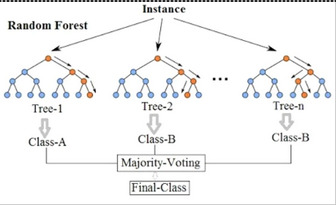
\includegraphics[width=2.5in]{figs/randon_forest.jpeg}
\caption{The Random Forest (RF) algorithm}
\label{fig_sim}
\end{figure}
In another study \cite{tesselle2024mlnet}, CNNs were used to detect soybean diseases, but challenges were encountered in distinguishing between visually similar disease symptoms, which may lead to misclassification. These issues highlight the importance of a robust and high-quality dataset, with well-labeled images that cover all possible variations. Nevertheless, CNNs can be effectively trained when the dataset is diverse and capable of capturing relevant visual nuances. 

 This study proposes a comparison between three different CNN architectures and the Random Forest model to evaluate their performance in phenological classification tasks. The goal is to identify the most effective approach for accurately classifying phenological stages, considering model accuracy, ease of implementation, and data requirements. The CNN models used—ResNet50, InceptionV3, and VGG16—were chosen due to their proven efficiency in various computer vision contexts. The Random Forest (RF) model was selected for its strong performance in classification tasks, interpretability, and lower susceptibility to overfitting. This comparison enables a comprehensive analysis to determine the most suitable tool for phenological stage classification in soybean crops. 
\begin{figure}[!h]
\centering
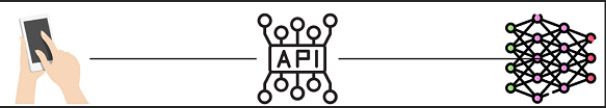
\includegraphics[width=2.5in]{figs/api.jpeg}
\caption{Integration between RF, API, and App}
\label{fig_sim}
\end{figure}
Before the training and the decision on the best classification technology to be integrated between the mobile app and the segmentation technology, the following technologies were used: 
\begin{itemize}
\item Flask: To create the API and manage HTTP requests.
\item TensorFlow: To load the machine learning model and make predictions. 
\item PIL (Pillow): For image manipulation. 
\item NumPy: For handling arrays and numerical data.
\end{itemize}
\section{Materials and Methods}
This research is experimental and applied in nature, with the objective of training three CNN network models and one RF model to compare the results and select the best solution for identifying the ideal moment for soybean crop desiccation. For the success of the study, it was necessary to collect images at different phenological stages, resulting in 10,000 soybean images from the Western region of Paraná, during the period from October 2024 to January 2025. The images were classified into two main groups: those in which the phenological stage was above R7 and those in which it was below R7. These classifications were essential for training the CNN and RF. 
\begin{figure}[!h]
\centering
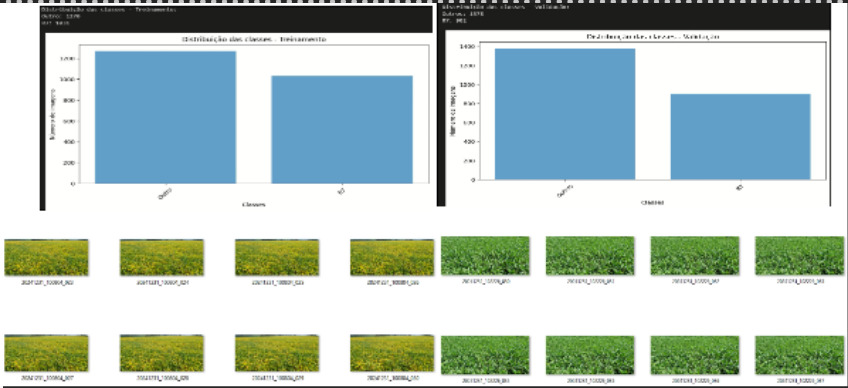
\includegraphics[width=2.5in]{figs/comparacion.jpeg}
\caption{Distribution of images in training and validation classes. }
\label{fig_sim}
\end{figure}
For the training of CNN and Random Forest (RF) models, 2,301 images of different phenological stages were selected for the training set and 2,280 images for the validation set, as illustrated in Fig. 1. These images played an important role in ensuring that the models were capable of generalizing and performing accurate classifications, especially regarding phenological stages above R7. The images were carefully captured, taking into consideration the need to avoid the presence of unwanted elements, such as shadows, trees, buildings, and sky, which could introduce noise and compromise the quality of the training. 
\begin{figure}[!h]
\centering

\includegraphics[width=2.5in]{figs/image_exemple.jpeg}
\caption{Implemented Neural Networks VGG16, Inception3, ResNet50.}
\label{fig_sim}
\end{figure}
Fig. 3 shows the implementation of the VGG16, Inception3, and ResNet50 CNNs. These CNN architectures are popular and contain particularities that make them different and are used for different types of image classification problems. VGGNet, developed by Simonyan and Zisserman in 2015, is a CNN architecture that exclusively uses 3×3 filters in its convolutional layers. The VGG16 version, composed of 16 layers, demonstrated high accuracy in image classification. However, its depth results in high memory consumption and significant computational demand \cite{goodfellow2016deep}. 
InceptionV3 is a more complex CNN, proposed by Google. The differential of this architecture lies in its use of Inception modules, which apply different filter sizes (such as 1x1, 3x3, 5x5) and dimensionality reduction techniques, such as 1x1 convolution, allowing the network to extract a greater number of features efficiently. The main advantage of InceptionV3 is its ability to balance accuracy and computational efficiency, making it faster and more effective compared to simpler networks, such as VGG16 \cite{akgun2023working}. Additionally, it is better able to handle images of different scales and contexts, making it useful for classifying complex images, such as those found in agricultural contexts. 
ResNet50 is one of the most innovative architectures, known for introducing residual blocks. These blocks allow information to flow directly from one layer to another, without the need for intermediate passages, which helps avoid the problem of network degradation. It is composed of 50 layers and was designed to handle extremely deep networks without losing performance. 
All three architectures (VGG16, InceptionV3, and ResNet50) were trained using an 80\% split for training and 20\% for testing. After training, a validation set was used to monitor the model's performance and adjust hyperparameters during the training process, ensuring that the model generalized well and was not merely overfitting to the training data. This approach helps ensure that the model learns the relevant characteristics of the data without losing its generalization capacity for new data.
\begin{figure}[!h]
\centering

\includegraphics[width=2.5in]{figs/image_exemple.jpeg}
\caption{Random Forest feature extraction model}
Random Forest, as illustrated in Fig. 4, is a machine learning model based on decision trees. It builds multiple trees and combines their results to obtain more robust predictions. \cite{kohersen2017random}

\label{fig_sim}
\end{figure}
\section*{Results and Discussion}
Table II presents the accurate results obtained for the training and validation datasets. 
\begin{table}[!h]
\renewcommand{\arraystretch}{1.3}
\caption{Model Accuracy}
\label{table:model_accuracy}
\centering
\begin{tabular}{|c|c|c|}
\hline
\textbf{Model} & \textbf{Training Accuracy (\%)} & \textbf{Validation Accuracy (\%)} \\
\hline
ResNet50 & 94.51 & 73.55 \\
\hline
InceptionV3 & 98.37 & 70.75 \\
\hline
VGG16 & 98.72 & 70.96 \\
\hline
Random Forest & 100.00 & 86.45 \\
\hline
\end{tabular}
\end{table}
% \caption{Comparison of training and validation accuracy among models.}

Although the convolutional neural network (CNN) models achieved high accuracy on the training set, their performance on the validation set was onsiderably lower, indicating the presence of overfitting. Overfitting occurs when a model learns the patterns of the training set too well and too quickly, which hinders its ability to generalize to unseen data. 

In contrast the decision tree-based model, Random Forest, achieved 100\% accuracy on the training set and also recorded the highest validation accuracy, demonstrating superior generalization capability. 

These results suggest that, despite the complexity and strong fitting performance of deep neural networks on training data, a traditional machine learning model may be more effective in terms of generalization, depending on the context and nature of the data. 
Furthermore, confusion matrices for the VGG16, ResNet50, and InceptionV3 models were analyzed to further evaluate the performance of these algorithms.
\begin{figure}[!h]
\centering

\includegraphics[width=2.5in]{figs/image_exemple.jpeg}
\caption{Confusion Matrix – ResNet50. }
\label{fig_sim}
\end{figure}
The ResNet50 model achieved a training accuracy of 94.51\%. However, its validation accuracy dropped to 73.55\%, suggesting potential overfitting on the training data. The confusion matrix for ResNet50, shown in Fig. 4, revealed a balanced distribution between the classes, with a correct classification rate of 42\% for the 'Other' class and 58\% for the 'R7' class. These results indicate challenges in accurate class identification, leading to suboptimal model performance. 
\begin{figure}[!h]
\centering

\includegraphics[width=2.5in]{figs/image_exemple.jpeg}
\caption{Confusion Matrix –  Incetion V3.  }
\label{fig_sim}
\end{figure}
The InceptionV3 model demonstrated excellent performance on the training dataset, achieving an accuracy of 98.37\%. However, the validation accuracy decreased to 70.75\%, indicating overfitting. As illustrated in Fig. 5, the confusion matrix shows a similar pattern to that of ResNet50, with a 41\% accuracy for the 'Other' class and 59\% for the 'R7' class. The false positive rate was 59\%, while the false negative rate was 41\%. InceptionV3 also struggles with distinguishing between classes, particularly in classifying instances of the 'Other' class. 
\begin{figure}[!h]
\centering

\includegraphics[width=2.5in]{figs/image_exemple.jpeg}
\caption{Confusion Matrix –  VGG16. }
\label{fig_sim}
\end{figure}
The VGG16 model achieved the highest training accuracy, with 98.72\%, and exhibited the lowest overfitting rate among the CNN models. However, its validation accuracy was 70.96\%, indicating that the model struggled to maintain strong performance on unseen data. These results suggest that while deep learning models such as ResNet50 and VGG16 performed well during training, their generalization capabilities still require improvement. 

As shown in Fig. 6, VGG16 yielded better classification performance for the 'R7' class, achieving a correct prediction rate of 67\%. However, for the 'Other' class, the accuracy was only 37\%. Although its performance in identifying 'R7' was superior, the false positive rate was 63\%, indicating that the model remains inadequate. Among the CNNs evaluated, VGG16 was slightly more effective in classifying the 'R7' growth stage. Nonetheless, all models demonstrated significant difficulty in accurately classifying the 'Other' class, with high false positive rates. To address these issues, future improvements may include hyperparameter tuning, data augmentation techniques, and rebalancing of the training dataset. 
\begin{figure}[!h]
\centering

\includegraphics[width=2.5in]{figs/image_exemple.jpeg}
\caption{Confusion Matrix –  Random Forest.}
\label{fig_sim}
\end{figure}
The trained Random Forest model exhibited strong performance, achieving 100\% training accuracy. This result may indicate overfitting. On the validation set, the model reached 86.45\% accuracy. As shown in Fig. 7, the model achieved a precision rate of 83.82\% for correctly idenfying negative instances (class 0 represents the "Other" class). The false positive rate for this class was 16.18\%. For positive instances (class 1, corresponding to “R7”), the precision was 93.02\%, and the false negative rate was 6.98\%. 
\begin{figure}[!h]
\centering

\includegraphics[width=2.5in]{figs/image_exemple.jpeg}
\caption{Final Training Results - Random Forest.}
\label{fig_sim}
\end{figure}
 

As depicted Fig. 8, the Random Forest model achieved 100.00\% training accuracy and 86.45\% validation accuracy. The classification report for the validation set includes precision, recal, and F1-score metrics for class 0 and 1, with respective values of 0.95, 0.82 and 0.88 for the 'Other' class, and 0.77, 0.94 and 0.85 for the 'R7' class. The o verall metrics include an accuracy of 0.86, as well as macro and weighted averages of 0.86/0.88/0.87 and 0.88/0.86/0.87 for precision/recall/F1-score, respectively. These results indicate that the model performs well overall, although its precision in validation is lower than in training. 
\section*{Conclusion }
The results obtained in this study highlight the importance of training multiple models for image classification tasks. While convolutional neural networks (CNNs) achieved high training accuracy, they demonstrated limitations in generalization. Validation accuracy ranged from 70.75\% (InceptionV3) to 73.55\% (ResNet50), indicating potential overfitting—where models effectively memorize the training set but struggle to perform on unseen data. 

In constrast, the Random Forest model, trained using features extracted from ResNet50, achieved 100\% accuracy on the training set and maintained superior validation performance (86.45\%), indicating better generalization capability. 

The analysis of the confision matrix f urther supports the effectiveness of the Random Forest model, which demonstrated a balanced trade-off between precision and recall. For the 'Other' class, the model achieved 95\% precision and 82\% recall, w hile for the “R7” class, precision and recall were 77\% and 94\%, respectively. These results indicate consistent performance in correctly classifying both positive and negative instances. 

In conclusion, although CNNs are highly effective for deep learning tasks, traditional machine learning models such as Random Forest—when combined with feature extraction techniques—can offer competitive performance, particularly in terms of generalization. Future research should explore strategies to mitigate overfitting in CNNs, including
\bibliographystyle{IEEEtran}
\bibliography{example} 

\end{document}


